%!TEX root = ../Thesis.tex

\chapter{Verwandte Arbeiten}
\label{cha:related_work}

Das folgende Kapitel gibt eine Überblick über einige wichtige und interessante wissenschaftliche
Arbeiten, welche sich mit der Analyse von Trajektoriedaten und insbesondere Fahrzeugtrajektorien beschäftigen.
Zu Beginn werden diverse Arbeiten vorgestellt, welche sich mit der Clusteranalyse von Trajektorien befassen.
Anschließend wird betrachtet, wie in der Literatur die Erkennung von Fahrspuren, vorzugsweise auf Basis
von Trajektorien, umgesetzt wird.
Zudem werden Arbeiten untersucht, welche sich bereits mit der Klassifizierung von Fahrspuren befassen. % TODO: Evtl. entfernen
Am Ende des Kapitels werden Defizite der existierenden Lösungen festgehalten und analysiert, welche
spezifischen Neuerungen für die Umsetzung dieser Arbeit nötig sind.

\section{Clusteranalyse von Trajektorien}
\label{sec:rw_clustering}
% Einleitung: Wichtigkeit und Informationsreichtum Trajektorien; Daher Analyse seit geraumer Zeit;
% In verschiedenen Anwendungsgebieten und mit unterschiedlichsten Zielen; Hier vorstellung verfahren, anhand dessen ersichtlich
% werden soll, wie probleme auf unterschiedliche Art gelöst werden.

Aufgrund der großen Menge an Informationen, welche sich auf Basis von Trajektoriedaten ermitteln lassen, ist ihre
Analyse schon seit geraumer Zeit Gegenstand wissenschaftlicher Untersuchungen.
Nachfolgend werden einige Arbeiten vorgestellt, welche sich mit der Clusteranalyse von Trajektorien beschäftigen.
Die Auswahl zeigt prototypisch, wie unterschiedliche die Anwendungsszenarien und Ziele bei solchen Analyse sind.

% Fu et al., 2005
\subsubsection*{Similarity based vehicle trajectory clustering and anomaly detection}
Eine Arbeit, welche ein sehr typisches Anwendungszenario behandelt, stammt von \cite[]{Hu2005}. Die Autoren
beschreiben in dieser Veröffentlichung ein Verfahren zur Clusteranalyse von Fahrzeugtrajektorien. Ziel dieser
ist es, auf Basis der entdeckten Spur-Cluster, anormale Verkehrsmanöver in Live-Aufnahmen von Straßenabschnitten
detektieren zu können. Solche Manöver sind beispielsweise ``Fahren abseits der üblichen Bahnen'' oder
``zu schnelles/langsames Fahren''.
Die Fahrzeugtrajektorien sind in dieser Arbeit als Sequenzen zwei-dimensionaler Punkte definiert.
Um diese zu gruppieren, setzen Hu et al. auf klassische Clusterverfahren und die Verwendung eines
einfachen, metrischen Distanzmaßes. Dieses Maß, bekannt als HU Distanz (siehe Abschnitt \ref{sec:hu_distance}),
vergleicht Trajektorien über den mittleren Abstand zwischen zusammengehörigen Punktpaaren.
Da dies nur zuverlässig möglich ist, wenn die Trajektorien einige Bedingungen erfüllen, müssen die
Autoren diese vorverarbeiten. Sie vereinheitlichen daher die Abstände der Punkte einer Trajektorie und erweitern
sie zudem in Richtung der Szenen-Grenzen.

% TODO: Figure anpassen
\begin{figure}[H]
    \centering
    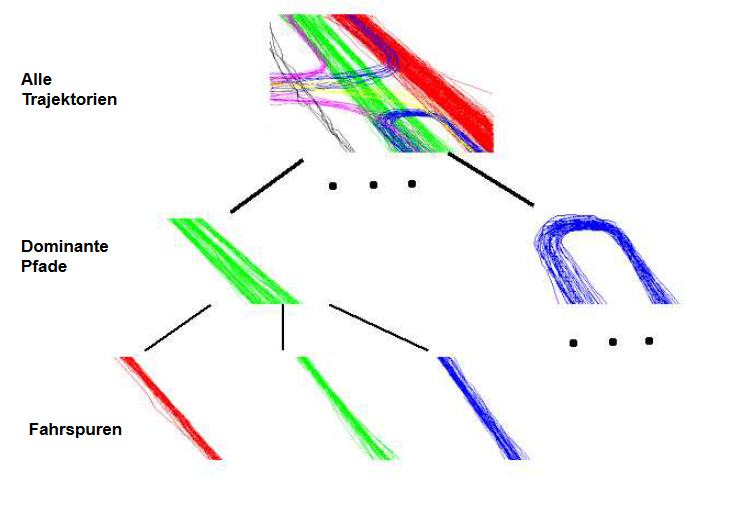
\includegraphics[width=0.5\linewidth]{../resources/img/RelatedWork/Fu_HierarchicalClustering}
    \caption[Zweistufiger Clustering-Vorgang von Hu et al.]{Zweistufiger Clustering-Vorgang von Hu et al. \cite[]{Hu2005}}
    \label{fig:relw_hu_two_step_cluster}
\end{figure}

Unter Verwendung des definierten Distanzmaßes werden die Trajektorien in einem zweistufigen Verfahren verarbeitet.
In den zwei Phasen werden, wie in Abbildung \ref{fig:relw_hu_two_step_cluster} dargestellt, zuerst dominante
Fahrpfade extrahiert, welche anschließend weiter in einzelne Fahrspuren untergliedert werden.
Als eigentliche Cluster-Algorithmen vergleichen die Autoren den \textit{Spectral-Clustering} Ansatz \cite[]{Ng2002}
mit einem \textit{Fuzzy-k-Means} Verfahren \cite[]{xie1991validity}.
Die Untersuchungen zeigen, dass der Spectral Clustering Ansatz nicht nur bessere Ergebnisse liefert, sonderen diese
über mehrere Durchläufe hinweg auch stabil sind, wohingegen die Resultate des Fuzzy-Ansatzes variieren.


% Junejo et al., 2004
\subsubsection*{Multi Feature Path Modeling for Video Surveillance}
Eine weitere Arbeit welche das Ziel hat, anormale Bewegungsmuster auf Basis von Trajektorien zu entdecken,
stammt von \cite[]{Junejo2004}. In diesem Fall geht es den Autoren allerdings nicht um das Finden von Fahrzeug-Fahrspuren,
sondern um die Extraktion von Laufpfaden von Fußgängern.
Die Bewegungsbahnen der Passanten werden aus Aufnahmen stationärer Überwachungskameras gewonnen und
als zwei-dimensionale Punktreihen repräsentiert.
Um die Trajektorien zu vergleichen, verwenden die Autoren die Hausdorff Distanz als Ähnlichkeitsmaß.
Die üblicherweise negativen Eigenschaften dieses
Vergleichkriteriums (siehe Abschnitt \ref{sec:hausdorff_distance}), konkret die Missachtung der
Trajektorie-Orientierung, sind bei diesem Anwendungsfall kein Nachteil sondern gewünscht.
Da Fußgänger auf einem Pfad oder Weg in entgegengesetzte Richtungen gehen können, muss die Orientierung
ihrer Trajektorien ignoriert werden.
Auf Basis der Hausdorff Distanz erstellen Junejo et al. einen vollständigen Graphen, in welchem die Knoten Trajektorien
und die gewichteten Kanten den Distanzen zwischen Trajektorien entsprechen.
Sie zerlegen diesen Graphen mit Hilfe eines rekursiven \textit{min-cut}-Graphen-Algorithmus, welcher sich
an der Arbeit von \cite[]{boykov2004experimental} orientiert, und erhalten so die Cluster für die
extrahierten Fußgänger-Trajektorien.

% Atev et al., 2010
\subsubsection*{Clustering of Vehicle Trajectories}
In der Arbeit \cite[]{Atev2010} ist das Ziel der Autoren, ein Verfahren zu finden, mit welchem Fahrzeugtrajektorien
bestmöglich gruppiert werden können, ohne diese im Voraus anpassen zu müssen.
Sie vergleichen hierzu die Performance von drei unterschiedlicher Distanzmaße unter Verwendung von zwei Cluster-Algorithmen.
Primäres Augenmerk legen die Autoren auf ein von ihnen bereits in \cite[]{Atev2006} entwickeltes Distanzmaß,
welches auf der Hausdorff Distanz basiert und sowohl die Orientierung von Trajektorien berücksichtigt
als auch robust gegenüber Ausreißern ist. Dieses neue Ähnlichkeitsmaß ist für zwei Trajektorien $P$ und $Q$
wie folgt definiert:

\begin{ceqn}
\begin{align}
    h_{\alpha, N, C}(P, Q) = \overset{\alpha}{\underset{p \in P}{ord}}\ \Big\{ \underset{q \in N_Q(C_{P,Q}(P))}{min} d(p, q) \Big\}
\end{align}
\end{ceqn}

Hierbei entspricht $C_{P,Q}$ einem Mapping $P \rightarrow Q$, welches einem Punkt $p \in P$ einen entsprechenden
Punkt $q \in Q$ zuweist, welcher die selbe relative Position in $Q$ besitzt wie $p$ in $P$.
$N_Q$ definiert ein Subset von $Q$ als Nachbarschaft des Punktes $q$. Zusammen definieren $N_Q$ und $C_{P,Q}$ eine
Struktur, in welcher der Abgleich der Trajektorien stattfindet. Dies ist visuell auch nochmals in Abbildung
\ref{fig:relw_atev_modh} dargestellt. Der Operator $ord_{p \in P}^{\alpha} f(p)$ selektiert jenen Wert aus $f(p)$, welcher
größer ist als $\alpha$-Prozent der Werte.

\begin{figure}[H]
    \centering
    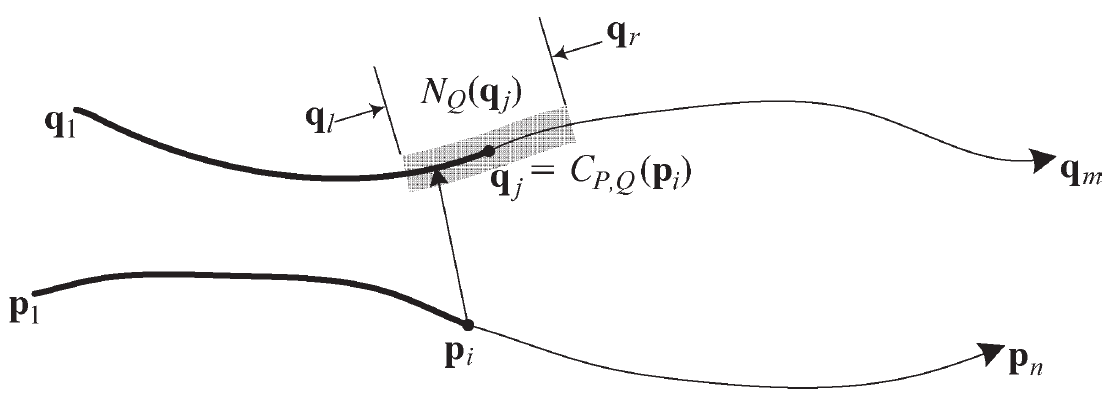
\includegraphics[width=0.6\linewidth]{../resources/img/RelatedWork/Atev_modHausdorff}
    \caption[Funktionsweise der modifizierten Hausdorff Distanz]{Funktionsweise der modifizierten Hausdorff Distanz \cite[]{Atev2010}}
    \label{fig:relw_atev_modh}
\end{figure}

Dank dieser Modifizierungen eignet sich das neue Ähnlichkeitsmaß gut für den Vergleich von Trajektorien:
$C_{P,Q}$ sorgt für den Einbezug der Orientierungen und über die Nachbarschaft $N_Q$ und $ord_{p \in P}^{\alpha} f(p)$
kann mit Ausreißern umgegangen werden.

Dieses Distanzmaß vergleichen Atev et al. unter Verwendung eines Spectral und eines Agglomerativen
Cluster-Algorithmus mit der \textit{Longest-Common Subsequence} (LCSS) und \textit{Dynamic Time Warping} (DTW) Distanz.
Die Ergebnisse der Untersuchungen für vier verschiedene Datensätze zeigen, dass die beste Cluster-Performance
mit Hilfe der modifizierten Hausdorff Distanz und des Spectral-Clustering erreicht wird.
Unter Verwendung der LCSS und DTW Distanzmaße, könnten die Autoren nicht die selben Resultate erzielen.

Dass das von Atev et al. vorgeschlagene Distanzmaß sehr gute Clusterergebnisse produziert, wurde auch von \cite{Morris2009}
bewiesen. In ihrer Untersuchung waren alledings die Ergebnisse, welche mithilfe des LCSS Maßes erreicht wurden,
ebenso gut, beziehungsweise teilweise sogar besser.

% Chen et al., 2011
\subsubsection*{Clustering of trajectories based on Hausdorff Distance}
Eine weitere interessante Arbeit zur Clusteranalyse von Trajektorien stammt von \cite[]{Chen2011}.
Die Autoren haben das Ziel, Muster in den Bewegungsbahnen von Hurrikans, welche im Zeitraum von 1850 bis 2010
über den Atlantik zogen, zu erkennen.
Sie verwenden hierzu einen angepassten DBSCAN Cluster-Algorithmus und das Hausdorff Distanzmaß.
Um die Missachtung der Orientierung kompensieren zu können, und zudem auch Ähnlichkeiten
in Sub-Trajektorien zu erkennen, wählen die Autoren eine etwas andere Darstellung der Trajektorien.
Sie definieren eine Bewegungsbahn als eine Folge sogenannter \textit{``Flow-Vektoren''}, welche neben
Positions- auch Richtungsinformationen enthalten. Ein solcher Vektor ist definiert über:

\begin{ceqn}
\begin{align}
    f_i = (x_i, y_i, dx_i, dy_i)
\end{align}
\end{ceqn}

wobei gilt:

\begin{ceqn}
\begin{align}
    dx_i = (x_{i+1} - x_i)/\sqrt{(x_{i+1} - x_i)^2 + (y_{i+1} - y_i)^2} \\
    dy_i = (y_{i+1} - y_i)/\sqrt{(x_{i+1} - x_i)^2 + (y_{i+1} - y_i)^2}
\end{align}
\end{ceqn}

Die Distanz zwischen zwei \textit{Flow-Vektoren} ist ihr euklidscher Abstand. Auf diese Weise wird bei
der Berechnung der Hausdorff Distanz (siehe Abschnitt \ref{sec:hausdorff_distance}) auch die Richtung
der Trajektorien berücksichtigt.
Um ähnliche Sub-Trajektorien entdecken zu können, teilen Chen et al. die Trajektorien an den Positionen
``charakteristischer'' Vektoren. Diese beschreiben Richtungsänderungen in einer
Bewegungsbahn und werden identifiziert über die Abweichungen in den Richtungskomponenten zweier
aufeinanderfolgender Flow-Vektoren. Dies ist anschaulich in Abbildung \ref{fig:relw_chen_flow_vector} dargestellt.

% TODO: Figure anpassen
\begin{figure}[H]
    \centering
    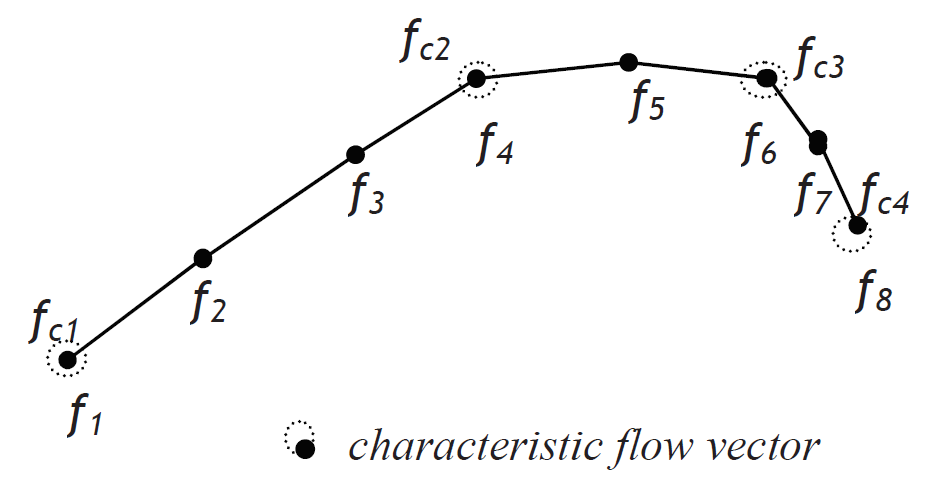
\includegraphics[width=0.45\linewidth]{../resources/img/RelatedWork/Chen_trajectory_splitting}
    \caption[Zerlegung einer Trajektorie in Sub-Trajektorien]{Zerlegung einer Trajektorie in Sub-Trajektorien \cite[]{Chen2011}}
    \label{fig:relw_chen_flow_vector}
\end{figure}

Die auf diese Weise erhaltenen Sub-Trajektorien werden von den Autoren mittels eines DBSCAN Algorithmus gebündelt.
Sie können so die üblichen Bewegungsbahnen von Hurrikans über dem Atlantik bestimmen.


% Vlachos et al., 2002
\subsubsection*{Discovering Similar Multidimensional Trajectories}
Die Arbeit \cite[]{Vlachos2002} thematisiert nicht direkt die Clusteranalyse von Trajektorien sondern
beschäftigt sich mit dem Vergleich von Bewegungsbahnen im drei-dimensionalen Raum. Konkret ist ihr Ziel,
Trajektorien vergleichen zu können, welche etwa die Handbewegungen beim Ausführen von Zeichensprache beschreiben.
Hierzu definieren die Autoren erstmals die Grundversion des LCSS Ähnlichkeitsmaßes, welches in vielen Arbeiten zum Einsatz
kommt \cite[]{Atev2006, Buzan2004, Chen2005}. Auf dessen Basis erstellen sie ein Distanzmaß, welche es ermöglicht
formgleiche aber im Raum verschobene Trajektorien zu finden.
Die Grundversion des LCSS Ähnlichkeitsmaßes und ein darauf basierendes einfaches Distanzmaß ist, nach Vlachos et al.,
bereits in Abschnitt \ref{sec:lcss_distance} definiert worden.
Dieses Maß erweitern die Autoren zudem wie folgt:

\begin{ceqn}
\begin{align}
    D2_{LCSS}(\delta, \epsilon, A, B) = 1 - \underset{f_{c,d} \in F}{max}\ D_{LCSS}(\delta, \epsilon, A, f_{c,d}(B))
\end{align}
\end{ceqn}

Hierbei ist $F$ eine Menge von Translations-Funktionen, welche die Trajektorien entlang der Achsen verschieben.
Sie besitzen die Form

\begin{ceqn}
\begin{align}
    f_{c, d}(A) = ((a_{x, 1} + c, a_{y, 1} + d), ..., (a_{x, n} + c, a_{y, n} + d))
\end{align}
\end{ceqn}

Abbildung \ref{fig:relw_vlachos_translation} veranschaulicht die Funktionsweise des Distanzmaßes. Es eignet sich immer dann, wenn Trajektorien
mit ähnlicher Form gefunden werden sollen, welche zudem eine gewisse räumliche Verschiebung aufweisen können.
Diese kann über die Größe von $F$ gesteuert werden.

\begin{figure}[H]
    \centering
    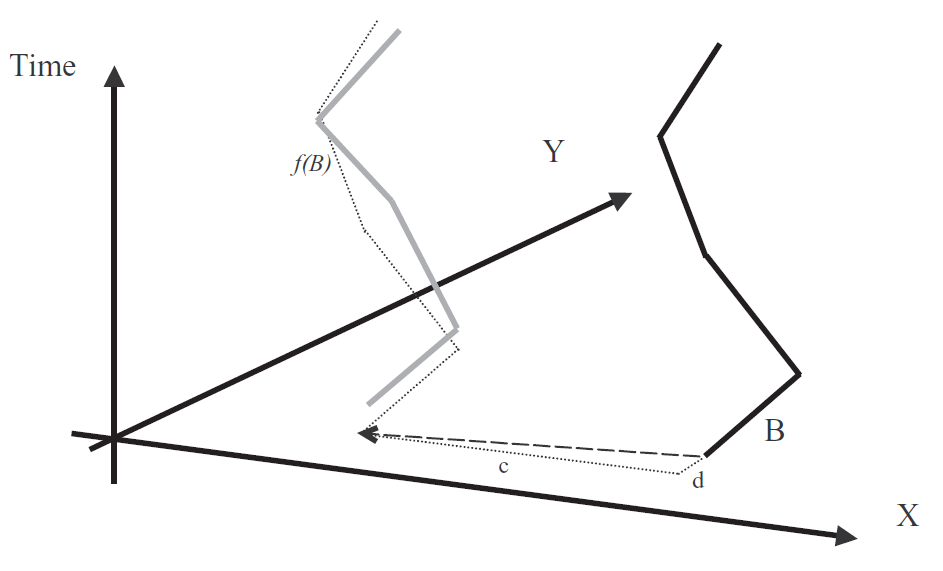
\includegraphics[width=0.55\linewidth]{../resources/img/RelatedWork/vlachos_translation}
    \caption[Verschiebung einer Trajektorie im Raum]{Verschiebung einer Trajektorie im Raum \cite[]{Vlachos2002}}
    \label{fig:relw_vlachos_translation}
\end{figure}

% Ren et al., 2014
\subsubsection*{Lane Detection in Video-Based Intelligent Transportation Monitoring via Fast Extracting and Clustering of Vehicle Motion Trajectories}

\cite[]{Ren2014} stellen in ihrer Arbeit ein interessantes Vorgehen zur Clusteranalyse von Trajektorien vor,
welches auf der \textit{Rough-Set}-Theorie beruht. Sie extrahieren Fahrzeugpositionen aus Aufnahmen stationärer
Überwachungskameras und stellen diese, wie die meisten Autoren, als Sequenzen zwei-dimensionaler
Punkte dar. Ihr Ziel ist anschließend, anhand einer Gruppierung der gewonnenen Fahrzeugtrajektorien,
die Spurmittelpunkte der Fahrbahnen zu bestimmen. Da ein nicht unerheblicher Anteil der Trajektorien Spurwechselvorgänge
enthält, welche eine Extraktion der Mittellinien erschweren, verwenden Ren et al. einen iterativen \textit{Rough-k-Means}
Algorithmus zur Clusterung der Trajektorien. Hierbei wird jedes Cluster über eine obere und untere Approximation beschrieben.
Die untere Approximation enthält dabei die Trajektorien, welche eindeutig der Spur zugeordnet werden können.
Die obere Näherung hingegen jene, welche Spurwechsel et cetera beschreiben. Bei der Berechnung der Spurmitten, werden
die Trajektorien der unteren Approximation höher gewichtet, als die der oberen. Ein sehr ähnlicher Cluster-Ansatz wurde
bereits in \cite[]{Lingras2004} vorgestellt.
Die initialen Mittellinien bestimmen die Autoren anhand einer \textit{Aktivitäts}- oder \textit{Heat}-Map,
welche sie während der Extraktion der Fahrzeugpositionen erstellen. Die Clusteranzahl $k$ muss händisch definiert werden.

Als Maß für die Distanz zwischen einer Trajektorie $A_x$ und einer Spurmitte $c_i$ verwenden Ren et al. die
Hausdorff Distanz $h(A_x, c_i)$. Für eine Trajektorie wird somit die nächste Mittellinie wie folgt gefunden:

\begin{ceqn}
\begin{align}
    h(A_x, c_m) = \underset{i = 1 ... k}{min}\ h(A_x, c_i)
\end{align}
\end{ceqn}

Hieraus ergibt sich die nachfolgende Definition für die Zuordnung der Bewegungsbahnen zu den Cluster-Näherungen:

\begin{ceqn}
\begin{align}
    \begin{cases}
        A_x \in \overline{C_m} \land A_x \in \overline{C_j} & \text{if } j \neq m \land \frac{h(A_x, c_j)}{h(A_x, c_m)} \leq \lambda \\
        A_x \in \underline{C_m} & \text{otherwise}
    \end{cases}
\end{align}
\end{ceqn}

Es gilt $1 \leq \lambda \leq 1.5$. $\overline{C_m}$ und $\underline{C_m}$ entsprechen der oberen und unteren
Näherung des $m$-ten Clusters und $\underline{C_m} \subseteq \overline{C_m}$.
Nachdem in jeder Iteration des Cluster-Vorgangs die Näherungen auf diese Weise bestimmt wurden, werden die neue Mittellinien
anhand Gleichung \ref{eq_ren_rough} errechnet.

\begin{ceqn}
\begin{align}
    \label{eq_ren_rough}
    c_i =
    \begin{cases}
        \frac{w_l \sum_{A_x \in \underline{C_i}} A_x}{|\underline{C_i}|} + \frac{(1 - w_l) \sum_{A_x \in (\overline{C_i} - \underline{C_i})} A_x}{|\overline{C_i} - \underline{C_i}|} & \text{if } \overline{C_i} \neq \underline{C_i} \\
        \frac{\sum_{A_x \in \underline{C_i}} A_x}{|\underline{C_i|}} & \text{otherwise}
    \end{cases}
\end{align}
\end{ceqn}

Als Gewichtungen $w_l$ verwenden Ren et al. Werte im Bereich $[0.5, 1]$. $| \cdot |$ entspricht hier der Kardinalität einer Menge.

Unter Verwendung dieser Clustering-Methode ist es den Autoren von \cite[]{Ren2014} möglich, auch bei einer hohen Anzahl von
Ausreißern und Spurwechselvorgängen, stabile Spurmittellinien zu bestimmen. Ergebnisse, welche dies zeigen, sind in Abbildung
\ref{fig:relw_ren_example_detection} dargestellt.

\begin{figure}[H]
    \centering
    \includegraphics[width=0.95\linewidth]{../resources/img/RelatedWork/ren_examples_detection}
    \caption[Ergebnisse der Spurmittellinien-Erkennung (Ren et al.)]{Ergebnisse der Spurmittellinien-Erkennung \cite[]{Ren2014}}
    \label{fig:relw_ren_example_detection}
\end{figure}


\section{Erkennung von Fahrspuren}
\label{sec:rw_lane_detection}
% Hier Arbeiten vorstellen, welche (prim. auf Basis von Traj.Clustern) versuchen Fahrspuren / Fahrbahnen
% zu erkennen
% Auch übliche Ansätze vorstellen, welche nicht mit Traj. arbeiten (erwähnen häufig optisch / aus Fahrzeugen)

Primäres Ziel dieser Arbeit ist es, Fahrspuren zuverlässig in Videoaufnahmen erkennen zu können. Dieser Abschnitt
geht daher auf einige Arbeiten ein, welche ähnliches ebenfalls versuchen.

Die Mehrzahl der Veröffentlichungen in diesem Bereich, löst das Problem, indem sie nach visuellen Merkmalen,
primär Spurtrennlinien, in Videoaufnahmen suchen. Die Aufnahmen werden dabei entweder von stationären Kameras,
von bemannten oder unbemannten Luftfahrzeugen oder einem Fahrzeug selbst gemacht. Zur Extraktion der Merkmale werden
üblicherweise Methoden aus den Gebieten des maschinellen Sehen (CV) oder maschinellen Lernens (ML) verwendet. % TODO: Abkzg.
Arbeiten, welche CV-basierte Ansätze verfolgen, stammen beispielsweise von \cite[]{Lai2000}, \cite[]{McCall2006} oder \cite[]{Aly2008}.
ML-gestützte Arbeiten wurden dahingegend unter anderem von \cite[]{Kim2008} und \cite[]{Gopalan2012} veröffentlicht.
% Ein mögliches Anwendungsgebiet für solche Ansätze ist Beispiel die Entwicklung eines Spurhalte-Assistenten.

Da oben genannte Ansätze, wie bereits zu Beginn der Arbeit erläutert, aufgrund von Verdeckungen oder Änderungen
in der Belichtung problematisch sind, werden nachfolgend ausschließlich Arbeiten vorgestellt, welche Fahrspuren
aus Trajektoriedaten extrahieren. Hierbei setzten die meisten als ersten Schritt auf eine Clusteranalyse von Trajektorien.
In der Repräsentation und Extraktion der Fahrspuren variieren die Ansätze hingegen.


% Fu et al. & Junejo et al.
%   Clustering und dann Bestimmung Envelopes basierend auf Varianz der Trajektorien in Cluster
\subsubsection*{A System for Learning Statistical Motion Patterns}
Die Arbeit \cite[]{WeimingHu2006} basiert auf dem bereits früher veröffentlichten Artikel \cite[]{Hu2005} der selben Autoren,
welcher oben beschrieben wurde. In dieser Publikation gehen Hu et al. nun genauer darauf ein, wie sie auf Basis
der Ergebnisse der Clusteranalyse, statistische Informationen über die Fahrbahnen der Fahrzeuge berechnen.
Hierzu wird für jedes Cluster zuerst eine Referenz-Trajektorie $T_r$ bestimmt. Dies ist jene Bewegungsbahn,
bei welcher die Summe der Distanzen zu allen anderen Trajektorien des Clusters minimal ist. Das verwendete
Distanzmaß ist hierbei des selbe, welches auch bei der Clusteranalyse zum Einsatz kam.
Die Autoren berechnen anschließend für jede Trajektorie-Gruppe eine Kette Gausscher-Wahrscheinlichkeits-Verteilungen
$\{ \varphi_1, \varphi_2, ..., \varphi_l \}$, wobei $l$ die Anzahl der Punkte der Referenz-Trajektorie ist.
Für jedes $\varphi_i$ wird der Mittelwert und die Kovarianz, basierend auf den Trajektorie-Punkten, welche dem
$i$-ten Punkt von $T_r$ am nächsten liegen, berechnet.
Anhand der Kovarianz Werte erstellen die Autoren Hüllen für die Fahrbahnen. Ergebnisse dieses Vorgehens sind in
Abbildung \ref{fig:relw_hu_example_envelope} dargestellt.

\begin{figure}[H]
    \centering
    \subfloat{{
        \includegraphics[width=0.49\linewidth]{../resources/img/RelatedWork/hu_example_envelope}
    }}
    \subfloat{{
        \includegraphics[width=0.49\linewidth]{../resources/img/RelatedWork/hu_example_envelope2}
    }}
    \caption[Spurhüllen in Hu et al., 2006]{Spurhüllen in \cite[]{WeimingHu2006}}
    \label{fig:relw_hu_example_envelope}
\end{figure}

Anzumerken ist, dass die extrahierten Spurhüllen nicht die tatsächliche Form, insbesondere die Breite, einer Fahrspuren
wiederspiegeln. Sie sind deutlich schmaler.


% Makris et al., 2005
\subsubsection*{Learning Semantic Scene Models From Observing Activity in Visual Surveillance}
% Erstellen Hüllen für Traj. --> Traj zu Bahn zuordnen
In \cite[]{Makris2005} extrahieren die Autoren übliche Bewegungsbahnen von Fußgängern aus stationären Videoaufnahmen.
Sie verwenden hierzu keine klassische Clusteranalyse, sondern ein iteratives und adaptives Online Verfahren,
welches neue Bewegungstrajektorien automatisch bestehenden Routen zuordnet oder neue initialisiert,
falls zu hohe Abweichungen zwischen der Trajektorie und den existierenden Bahnen bestehen.
Routen definieren Makris et al. hierbei als eine Sequenz von Knoten, welche folgende Merkmale besitzen:

\begin{itemize}
    \item 2D-Mittelpunkt
    \item Gewichtung (Anzahl der Trajektorien im Bereich des Knoten)
    \item Zwei Hüll-Punkte (Maximale- beziehungsweise Standardabweichung der Trajektorien der Route im Bereich des Knoten)
\end{itemize}

Abbildung \ref{fig:relw_hu_example_envelope} a) veranschaulicht nochmals die Definition einer Route.
Um aus einfachen Bewegungsbahnen Routen zu erstellen, verwenden die Autoren das nachfolgend beschriebene Verfahren,
welches dem agglomerativen Cluster-Ansatz ähnelt.

\begin{enumerate}
    \item Erste Trajektorie initialisiert erste Route
    \item Neue Trajektorien werden mit bestehenden Bahnen abgeglichen
    \begin{enumerate}
        \item Bei Übereinstimmung wird Route aktualisiert
        \item Bei keiner Übereinstimmung wird neue Route erzeugt
    \end{enumerate}
    \item Aktualisierte Routen werden auf definierten Knotenabstand $r$ gebracht
    \item Alle Routen werden miteinander verglichen
    \begin{enumerate}
        \item Bei Überlagerung der Routen werden diese fusioniert
    \end{enumerate}
\end{enumerate}

Als Vergleichsmaß für die Trajektorien und Routen, verwenden Makris et al. die maximale Distanz zwischen einer Trajektorie und
einer Routen-Hülle. Diese muss sich unterhalb eines bestimmten Grenzwertes befinden.
Ein Ergebnis des Verfahrens ist in Abbildung \ref{fig:relw_hu_example_envelope} b) dargestellt.

% TODO: Bild updaten
\begin{figure}[H]
    \centering
    \subfloat[]{{
        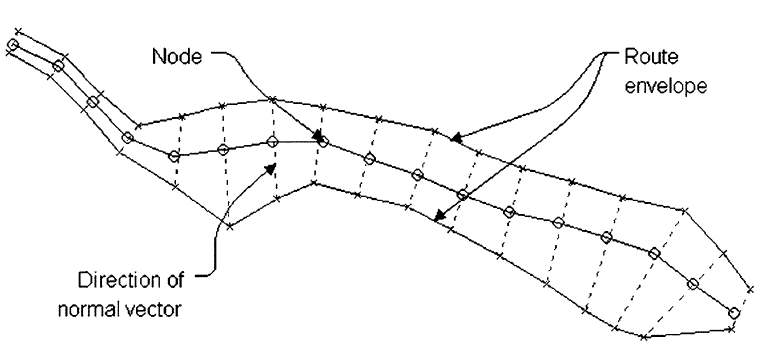
\includegraphics[width=0.49\linewidth]{../resources/img/RelatedWork/makris_route}
    }}
    \subfloat[]{{
        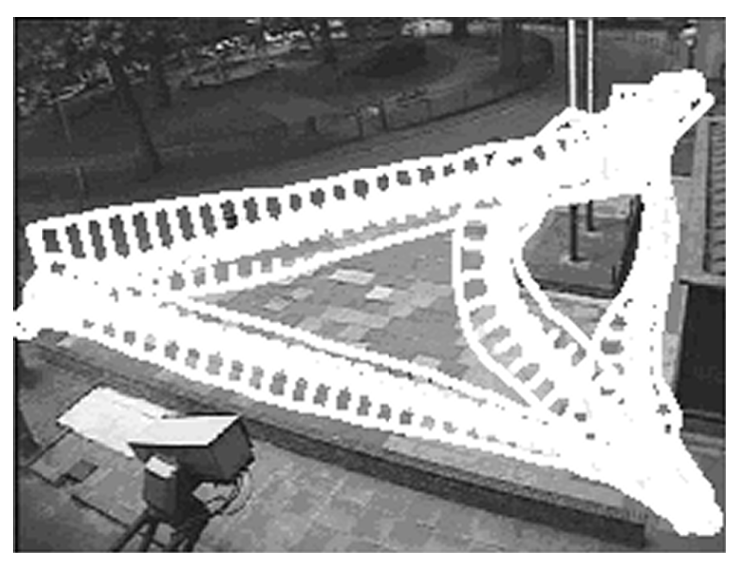
\includegraphics[width=0.49\linewidth]{../resources/img/RelatedWork/makris_result}
    }}
    \caption[Routen-Definition und Ergebnisse Routen-Erkennung (Makris et al.)]{a) Routen Definition, b) Ergebnisse Routen-Erkennung \cite[]{Makris2005}}
    \label{fig:relw_hu_example_envelope}
\end{figure}


% Morris et al., 2011
\subsubsection*{Trajectory Learning for Activity Understanding: Unsupervised, Multilevel, and Long-Term Adaptive Approach}
% HMM


% Hsieh et al., 2006
\subsubsection*{Automatic Traffic Surveillance System for Vehicle Tracking and Classification}
% Heat Map --> Spurmittellinien --> Begrenzer aus Mittellinien bestimmen

\cite[]{Hsieh2006} stellen in ihrer Arbeit ein System zur Extraktion von Fahrzeugpositionen aus Aufnahmen
stationärer Verkehrskameras vor. Auf diesen aufbauend definieren sie einen Algorithmus, mit dessen Hilfe es
möglich ist, Spurmittel- und Begrenzungs-Linien zu entdecken.
Hierzu erzeugen Hsieh et al. ein Histogramm $H_{vehicle}(x,y)$, welches die Häufigkeit abbildet, das ein Fahrzeug sich über eine
bestimmte Pixel-Position $(x, y)$ bewegt. Ein solches ist in Abbildung \ref{fig:relw_hsieh_results} a) dargestellt.
Die Autoren gehen davon aus, dass die Fahrzeugpositionen sich mehrheitlich in der Mitte einer Spur befinden und
ein Histogramm, welches für eine Fahrbahn mit $L_n$ Spuren erstellt wurde, $L_n$ Maxima in jeder Zeile besitzt,
welche die Spurmitten darstellen.
Sie isolieren daher die Maxima in $H_{vehicle}$ als Mittellinien. Es sei anschließend $C_{L_k}^{j}$ die $k$-te Spurmittellinie
in Zeile $j$ des Histogramms. Daraus berechnen Hsieh et al. die Spurbegrenzungslinien. Alle innen liegenden
Begrenzungen ergeben sich aus Gleichung \ref{eq_hsieh1}. $DL_{k}^{j}$ entspricht hierbei einem Punkt
in der $j$-ten Reihe der $k$-ten Begrenzung.

\begin{ceqn}
\begin{align}
\label{eq_hsieh1}
    DL_{k}^{j} = \frac{1}{2} (C_{L_{k-1}}^{j} + C_{L_{k}}^{j})
\end{align}
\end{ceqn}

Die Breite $w_{L_k}^{j}$ der $k$-ten Fahrspur ergibt sich zudem wie folgt:

\begin{ceqn}
\begin{align}
\label{eq_hsieh2}
    w_{L_k}^{j} = | C_{L_{k}}^{j} - C_{L_{k-1}}^{j} |
\end{align}
\end{ceqn}

Die Positionen der äußeren Spurbegrenzungen einer Fahrbahn ergeben sich für die $j$-te Zeile des Histogramms
aus den Gleichungen \ref{eq_hsieh3} und \ref{eq_hsieh4}.

\begin{ceqn}
\begin{align}
\label{eq_hsieh3}
    (x_{DL_0^j}, j) &= (x_{DL_1^j - w_{L_0}^j}, j) \\
\label{eq_hsieh4}
    (x_{DL_{N_L}^j}, j) &= (x_{DL_{N_{L-1}}^j + w_{L_0}^j}, j)
\end{align}
\end{ceqn}

Ein Beispiel für die Ergebnisse der Spurerkennung von Hsieh et al. ist in Abbildung \ref{fig:relw_hsieh_results} b) dargestellt.
Das Verfahren funktioniert grundlegend gut, wenn Fahrspuren nebeneinader und parallel zueinander liegen.

\begin{figure}[H]
    \centering
    \subfloat[]{{
        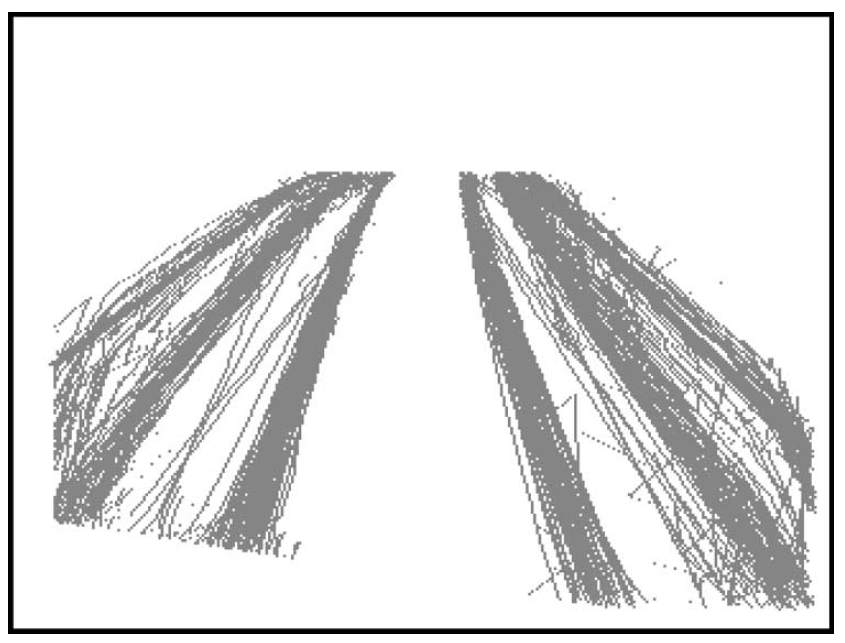
\includegraphics[width=0.33\linewidth]{../resources/img/RelatedWork/hsieh_histogram}
    }}
    \subfloat[]{{
        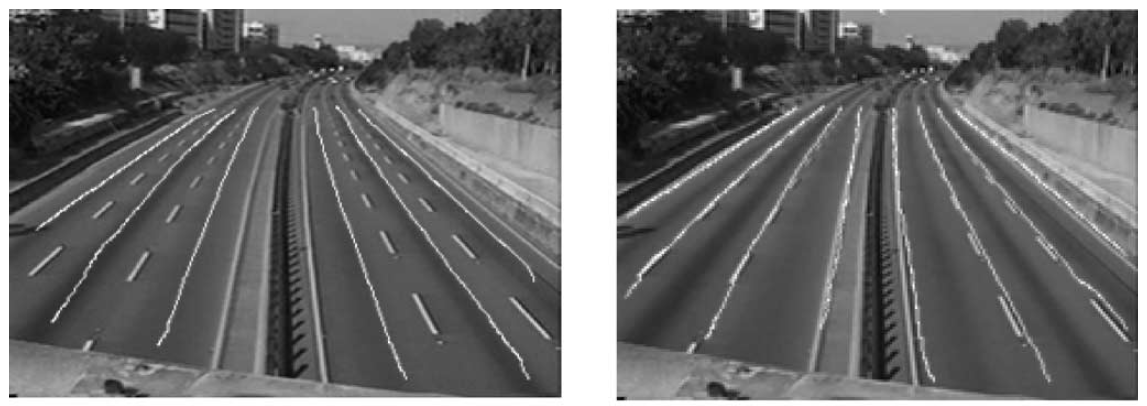
\includegraphics[width=0.68\linewidth]{../resources/img/RelatedWork/hsieh_centers_and_borders}
    }}
    \caption[Ergebnisse Histogramm Erstellung und Spurextraktion (Hsieh et al.)]{a) Fahrzeugpositions Histogramm, b) Spurmittellinien und Spurbegrenzungslinien \cite[]{Hsieh2006}}
    \label{fig:relw_hsieh_results}
\end{figure}


\section{Defizite vorhandener Lösungen und benötigte Neuerungen}
\label{sec:rw_deficites}

% Eigentlich nichts zur Spurerkennung auf bspw. Kreuzungen etc.
%   Wenn Spur dann immer nur Spur für gesamtes Cluster (kein Partitioning)

% Meiste Aufnahmen sind Frontal-Aufnahmen auf Straße --> keine Verzerrungen